\chapter{RSSp}



\section{Introduction}\label{sec:org3c6cf58}


There is no concept more central to the study of genetics than that of heritability. In the simplest definition, a trait is heritable if offspring are more similar to their parents (in regards to the trait) than they are to random members of the same population. Narrow-sense heritability, or $h^2$ is the proportion of a trait's variance that can be attributable to additive genetic variance. 
$h^2$ has traditionally been measured by studying twins or pedigress, but can be biased when assumptions about the sources of phenotypic covariance are violated\cite{keller2005quantifying}.
Over the last decade or so, SNP-based methods have been developed\cite{gcta} and widely applied to the problem of $h^2$ estimation, based on large scale genome-wide association studies (GWAS). 
%As methods for estimating $h^2$ using whole-genome data
%In the case of most complex traits, the most strongly associated genetic variants collectively explain a relatively small fraction of the total trait variation that is thought to be attributable to genetics.
These methods leverage information of variants across the genome, rather than only strongly associated variants, which explain only a small fraction of heritability estimated from twin studies.  
%A consistent frustration of the human geneticist is that the total explanatory power of strongly associated variants is often small compared to what heritability estimates from twin studies.
The state of art method for estimating heritability using genotype and phenotype data of unrelated individuals is Genome-based restricted maximum likelihood (GREML)\cite{GCTA}. GREML has been used to great effect to explain a large proportion of heritability found by family studies \cite{GCTA}. These methods, however, requires individual-level data, which can be difficult to access, as well as the construction of an $n \times n$ relatedness matrix (with $n$ being the number of individuals).  The size of this matrix increases quadratically as sample size increases, raising substantial computational burden.
The latest methods for heritability estimation often use GWAS summary statistics, in the form of the estimated effect sizes and standard errors, and p-values, of marginal association of each variant. Summary statistics have become the most common method for summarizing and storing estimated relationships between genotype and phenotype \cite{Lyon_2020}.
%As such, they have become an invaluable resource for a large number of biomedical research applications\cite{Lyon_2020}.  
There are many advantages of working with summary statistics, comparing with individual level data, including: easier comparison of genetic-association signal across traits at a locus\cite{phewas}, across loci for a trait\cite{firstGWAS}, and the comparison of patterns of genotype-phenotype associations across populations\cite{Rosenberg_2010}.
%In the Bayesian setting this stat and among the most important.  
%Among the most important applications of GWAS sumamry statistics is in the estimation of heritability. 
LD score regression is the most widely used method for estimating heritability from GWAS summary statistics.  LD score regression uses GWAS summary statistics and an estimate of the linkage disequilibrium (LD) between those variants to estimate the heritability of the trait as well as the extent of confounding in the GWAS\cite{ldsc}. Other summary statistics based methods, e.g. LDAK-SumHer, allows more complex relationship of the effect sizes of variants and their minor allele frequencies (MAF) and LD structure. 

%A key component of heritability estimation methods using GWAS summary statistics is a statistical model relating the marginal, variant-level associations between genotype and phenotype to the distribution of true effect sizes. 
%Among the state of the art methods for the estimation of heritability from 

All the summary statistics based methods for heritability estimation, however, are essentially method-of-moment estimators. These methods often use ad-hoc procedures to deal with dependency of nearby variants due to LD. A full likelihood based model for parameter estimation, while accounting for LD among variants, would be statistically optimal. Our work takes advantages of the likelihood model developed by our collaborators, known as Regression with Summary Statistics (RSS)\cite{Zhu_2017}, in modeling the relationship between marginal associations of single variants and the true effect sizes of all variants. Here we present a model with RSS likelihood with a normal prior distribution of effect sizes, which we call polygenic RSS, or RSSp. We come up with a computationally efficient technique to make inference under RSSp. Additionally, we estimate heritability, not as a single unknown parameter, but using the sum of Percent of Variance Explained (PVE) of all individual SNPs, a strategy that makes the results less sensitive to the prior assumption. 
Using simulation, we show under truly polygenic genetic architectures, RSSp is able to better estimate heritability than LD score regression.
We also explore the consequences of using an out-of-sample reference LD from external data to demonstrate the importance of accurate estimation of linkage disequilibrium and explore how shrinkage estimators of LD can improve estimates of heritability.  

\section{Background}

The most common method for associating genotype with phenotype is through  an additive model:

$$ \textbf{y}= \textbf{X} \boldsymbol{\beta} + \boldsymbol{\epsilon}$$

where $\textbf{y}$ is the length $n$ vector of phenotypes, \(X\) is an (\(n\) by \(p\)) matrix representing genotype, (which we will assume is centered for mathematical convenience, and without loss of generality), \(\boldsymbol{\beta}\) is a vector (length \(p\)) of variant-level effects and \(\epsilon\) is noise/error. In this model, the narrow sense heritability is defined as $h^2=\frac{\text{Var}(\textbf{X}\boldsymbol{\beta})}{\text{Var}(\boldsymbol{\epsilon})}$. With current GWAS sample sizes the number of variants is much larger than the number of samples \(i.e. p >>n\), so it is difficult or even impossible to estimate $\beta_j$ for each variant $j$, so $\boldsymbol{\beta}$ is often treated as a random variable, following some prior distribution. %leading to  $\boldsymbol{\epsilon} = \textbf{y}-\textbf{X}\boldsymbol{\beta} \rightarrow \text{Var}(\boldsymbol{\epsilon})= \text{Var}(\textbf{y})-\text{Var}(\textbf{X}\boldsymbol{\beta})$.  
In a GWAS context $\textbf{X}$ and $\textbf{y}$ are fixed, which means that estimating $h^2$, \emph{for the population from which the sample is drawn} can be reduced to estimating the distribution parameter(s) of $\beta$. %$\text{Var}(\boldsymbol{\beta})$.

The most common means of summarizing the results of a GWAS is to use GWAS summary statistics.
The summary statistics we will be interested in are the marginal effect size at a particular variant (\(j\)), which we will denote as
\(\hat{\beta_j}\), and the standard error of that estimate, which we will denote as \(\hat{\sigma_j^2}\). The estimates and standard errors are usually from simple regression of $Y$ against $X_j$, genotype of variant $j$: 

$$ \hat{\beta_j} := {({X_j}^{T}X_j)}^{-1}{X_j}^{T}y $$

$$ \hat{\sigma_j^2} := (nX_j^TX_j)^{-1}(y-X_j\hat{\beta_j})^T(y-X_j\hat{\beta_j}) $$

%Under such a regime we cannot directly estimate the distribution of \(\beta_i\).

\subsection{Regression with Summary Statistics RSS}\label{sec:orgb0b15e2}

RSS relates marginal association statistics to effect sizes $\boldsymbol{\beta}$ by using the LD matrix:

$$ \hat{\boldsymbol{\beta}} | \boldsymbol{\beta} \sim N(\hat{S}\hat{R}\hat{S}^{-1},\hat{S}\hat{R}\hat{S}) $$

where \(\hat{\boldsymbol{\beta}}\) is the length $p$ vector of GWAS effect size estimates,  $\hat{\textbf{S}}$ is a diagonal matrix where $\hat{S_{j,j}}=\hat{\sigma_j^2}$, and $\hat{R}$ is the LD matrix between variants, assuming variants are normalized (i.e. mean 0, variance 1). 

In the original RSS paper there were two priors on \(\beta\) that were discussed.  The first is based on the Bayesian Sparse Linear Mixed Model (BSLMM)\cite{bslmm} where true effects ($\boldsymbol{\beta}$)
come from a mixture of sparse and polygenic components:

$$ \beta_j \sim \pi N(0,\sigma^2_B+\sigma^2_P)+(1-\pi) N(0,\sigma^2_P) $$

Here \(\sigma^2_B\) represents the variance of the sparse component, while \(\sigma^2_P\) represents the variance of the polygenic component. Fitting the RSS model with this prior is quite computationally demanding, 
as the MCMC requires computing the multivariate normal density function, which itself requires cholesky decomposition of a \(p \times p\) matrix, an \(O(p^3)\) operation.  If one assumes that \(\sigma^2_P=0\),
i.e that there is no polygenic component, one arrives at the BVSR model:

$$ \beta_j \sim \pi N(0,\sigma^2_B)+(1-\pi) \delta_0 $$

The posterior for the BVSR model can be efficiently approximated using variational inference. 

If instead of assuming that \(\sigma^2_P=0\), one instead assumes that \(\sigma_B=0\) (or equivalently that \(\pi=0\)) we arrive at the following model: 
$$ \beta_j \sim N(0,\sigma^2_P)$$

With a normal prior (rather than a mixture of two normal distributions) and multivariate normal likelihood, we can write down the analytic form of the marginalized likelihood as shown below.

In general,if we know that the marginal Gaussian distribution for some variable \(\textbf{x}\) and a conditional Gaussian distribution for some \(\textbf{y}|\textbf{x}\) of the forms:
$$p(\textbf{x}) = N(\textbf{x}|\boldsymbol{\mu},\Lambda^{-1})$$

$$p(\textbf{y}|\textbf{x}) = N(\textbf{y}|A\textbf{x}+\textbf{b},L^{-1})$$
then the marginal distribution of \(\textbf{y}\) and the conditional distribution of \(\textbf{x}\) given \(\textbf{y}\) arge given by \cite{patternrecognition}: 

$$ p(\textbf{y}) = N(\textbf{y}|A\boldsymbol{\mu}+\textbf{b},L^{-1}+A\Lambda^{-1}A^{T})$$
$$p(\textbf{x}|\textbf{y}) = N(\textbf{x}| \Sigma \left\{ A^{T} L ( \textbf{y} - \textbf{b} ) + \Lambda \boldsymbol{\mu} \right\} , \Sigma)$$

where :
$$\Sigma = (\Lambda + A^{T}LA)^{-1}$$

Given this result, we can derive the posterior for \(\boldsymbol{\beta}\).

Remember that the prior for \(\boldsymbol{\beta}\) is \(\boldsymbol{\beta} \sim N(0,I_p\sigma^2_\beta)\), and that the RSS likelihood is \(\hat{\boldsymbol{\beta}} | \boldsymbol{\beta} \sim N(\hat{S}\hat{R}\hat{S}^{-1}\boldsymbol{\beta},\hat{S}\hat{R}\hat{S})\).  
We can replace \(\boldsymbol{\beta}\) with \(\textbf{x}\) and \(\hat{\boldsymbol{\beta}}\) with \(\textbf{y}\) by making the following substitutions:

\begin{center}
\begin{tabular}{ll}
Symbol & Replacement\\
\hline
\(\boldsymbol{\mu}\) & \(0\)\\
\(b\) & \(0\)\\
\(\Lambda^{-1}\) & \(I_p \sigma^2_\beta\)\\
\(A\) & \(\hat{\textbf{S}}\hat{\textbf{R}}\hat{\textbf{S}}^{-1}\)\\
\(L^{-1}\) & \(\hat{\textbf{S}}\hat{\textbf{R}}\hat{\textbf{S}}\)\\
 & \\
\end{tabular}
\end{center}

We then see that the distribution of \(\hat{\boldsymbol{\beta}}\) after marginalizing over $\boldsymbol{\beta}$ is:

$$ \hat{\boldsymbol{\beta}}|\sigma_\beta^2 \sim N(0,\sigma_\beta^2\hat{\textbf{S}}\hat{\textbf{R}}\hat{\textbf{S}}^{-1}\hat{\textbf{S}}^{-1}\hat{\textbf{R}}\hat{\textbf{S}}+\hat{\textbf{S}}\hat{\textbf{R}}\hat{\textbf{S}})$$ 

We can rewrite this as :
$$\hat{\boldsymbol{\beta}}|\sigma_\beta^2 \sim  N(0,\sigma_\beta^2\hat{\textbf{S}}\hat{\textbf{R}}\hat{\textbf{S}}^{-2}\hat{\textbf{R}}\hat{\textbf{S}}+\hat{\textbf{S}}\hat{\textbf{R}}\hat{\textbf{S}}) $$

Computing the marginalized likelihood in this case, though involving only a single parameter, requires an expensive recalculation of the multivariate normal probability density function, in particular 
the recomputation of the determinant and inverse of \(\sigma_\beta^2\hat{\textbf{S}}\hat{\textbf{R}}\hat{\textbf{S}}^{-2}\hat{\textbf{R}}\hat{\textbf{S}}+\hat{\textbf{S}}\hat{\textbf{R}}\hat{\textbf{S}}\) for each value of 
\(\sigma_\beta^2\).  A common computational trick for recomputing a multivariate normal density is to precompute a cholesky decomposition of the covariance matrix, as the computationally expenensive aspects of computing the multivariate normal density (in particular computing the determinant and inverse of the covariance matrix) have efficient implementations when the covariance matrix has been cholesky-decomposed.  This trick is unforunately not applicable in this situation.  Even if both $\hat{\textbf{S}}\hat{\textbf{R}}\hat{\textbf{S}}^{-2}\hat{\textbf{R}}\hat{\textbf{S}}$ and $\hat{\textbf{S}}\hat{\textbf{R}}\hat{\textbf{S}}^{-2}\hat{\textbf{R}}\hat{\textbf{S}}$ were factored separately, there is no way to add the two matrices to maintain the cholesky form.


\subsubsection{Polygenic RSS (\texttt{RSSp})}\label{sec:org040cb73}

If instead of modeling \(\hat{\boldsymbol{\beta}}\) and \(\boldsymbol{\beta}\), we can instead model $\hat{\textbf{u}}$ and $\textbf{u}$, where $\hat{u}_j=\frac{\hat{\beta_j}}{\hat{\sigma_j^2}}$, and  \(u_j=\frac{\beta_j}{\hat{\sigma_j^2}}\).  This is effectively the same as effect-size in terms of standardized genotypes, and leads to the same (implicit) prior as LD score regression\cite{ldsc} and GCTA\cite{GCTA}.  With the prior $\textbf{u} \sim \mathcal{N}(0,\sigma_u^2)$, the likelihood in terms of $\textbf{u}$ becomes:

$$\hat{\textbf{u}} | \textbf{u} \sim \mathcal{N}(\textbf{R} \textbf{u},\textbf{R})$$

, the marginalized form of $\hat{\textbf{u}}$ is:

\[ \hat{\textbf{u}}|\sigma_u^2 \sim N(0,\sigma_u^2\textbf{R}^2+\textbf{R})\]

Unlike the marginalized likelihood without the normalized-genotype assumption,
precomputing a matrix decomposition for the covariance matrix will greatly
accelerate efficient computation of the likelihood
and as a consequence, parameter estimation.
If we take the eigenvalue decomposition of $\textbf{R}$ $\textbf{R}=\textbf{Q}\textbf{D}\textbf{Q}^T$, with $\textbf{Q}$ 
being the $p$ by $p$ matrix of
eigenvectors, and $\textbf{D}$ being the diagonal matrix of eigenvalues, we can rewrite the marginalized likelihood as
$\hat{\boldsymbol{\beta}} \sim N(0,\sigma_u^2\textbf{QD}^2\textbf{Q}+\textbf{QDQ})$.  Letting
$\hat{\textbf{v}} = Q^{T}\hat{u}$, and exploiting the property of
the multivariate normal distribution that an affine transformation of a multivariate normal random variable has a multivariate normal distribution, the
likelihood for $\hat{\textbf{v}}$ is $\hat{\textbf{v}}|\sigma_u^2 \sim \mathcal{N}(0,\sigma_u^2\textbf{D}^{2}+\textbf{D})$.  As all the off-diagonal terms of
the covariance matrix for ${\textbf{v}}$ are $0$, we can equivalently write the likelihood for ${\textbf{v}}$ as the joint probability of $p$ independent
univariate normal variables where:

\[ v_j \sim N(0,\sigma^2_u\lambda_j^2+\lambda_j) \]

Computing the marginalized-likelihood estimate of $\sigma^2_u$ in terms of $\textbf{v}$ and $\textbf{D}$ can be done without the costly covariance inverse or determinant calculations required in the original multivariate probability density function.  We estimate $\sigma^2_u$ by the ``Brent'' 1D optimization routine in R\cite{brent1972algorithms}. 


\subsection{Linkage disequilibrium}\label{sec:org828aaeb}

Two genome-wide Linkage Disequilibrium (LD) estimates were generated.  The first, which we will refer to as ``in-sample'', was generated from same samples used to simulate phenotypes and subsequently generated GWAS summary statistics.  The second set we will refer to as ``reference-panel'', which is the equally sized set of individuals not used in generating GWAS summary statistics.  Rather than computing and storing 8 million by 8 million genome-wide LD matrix, a blockwise diagonal approximation to the LD matrix was made.  LD between variants was only estimated for variants within 1,703 approximately independent LD blocks.  The boundaries of independent LD blocks were previously identified in the 1000 genomes EUR population using the method ldetect\cite{ldetect}.  

\section{Results}\label{sec:org26555b8}

\begin{figure}
  \centering
  \begin{subfigure}[t]{\textwidth}
    \centering
    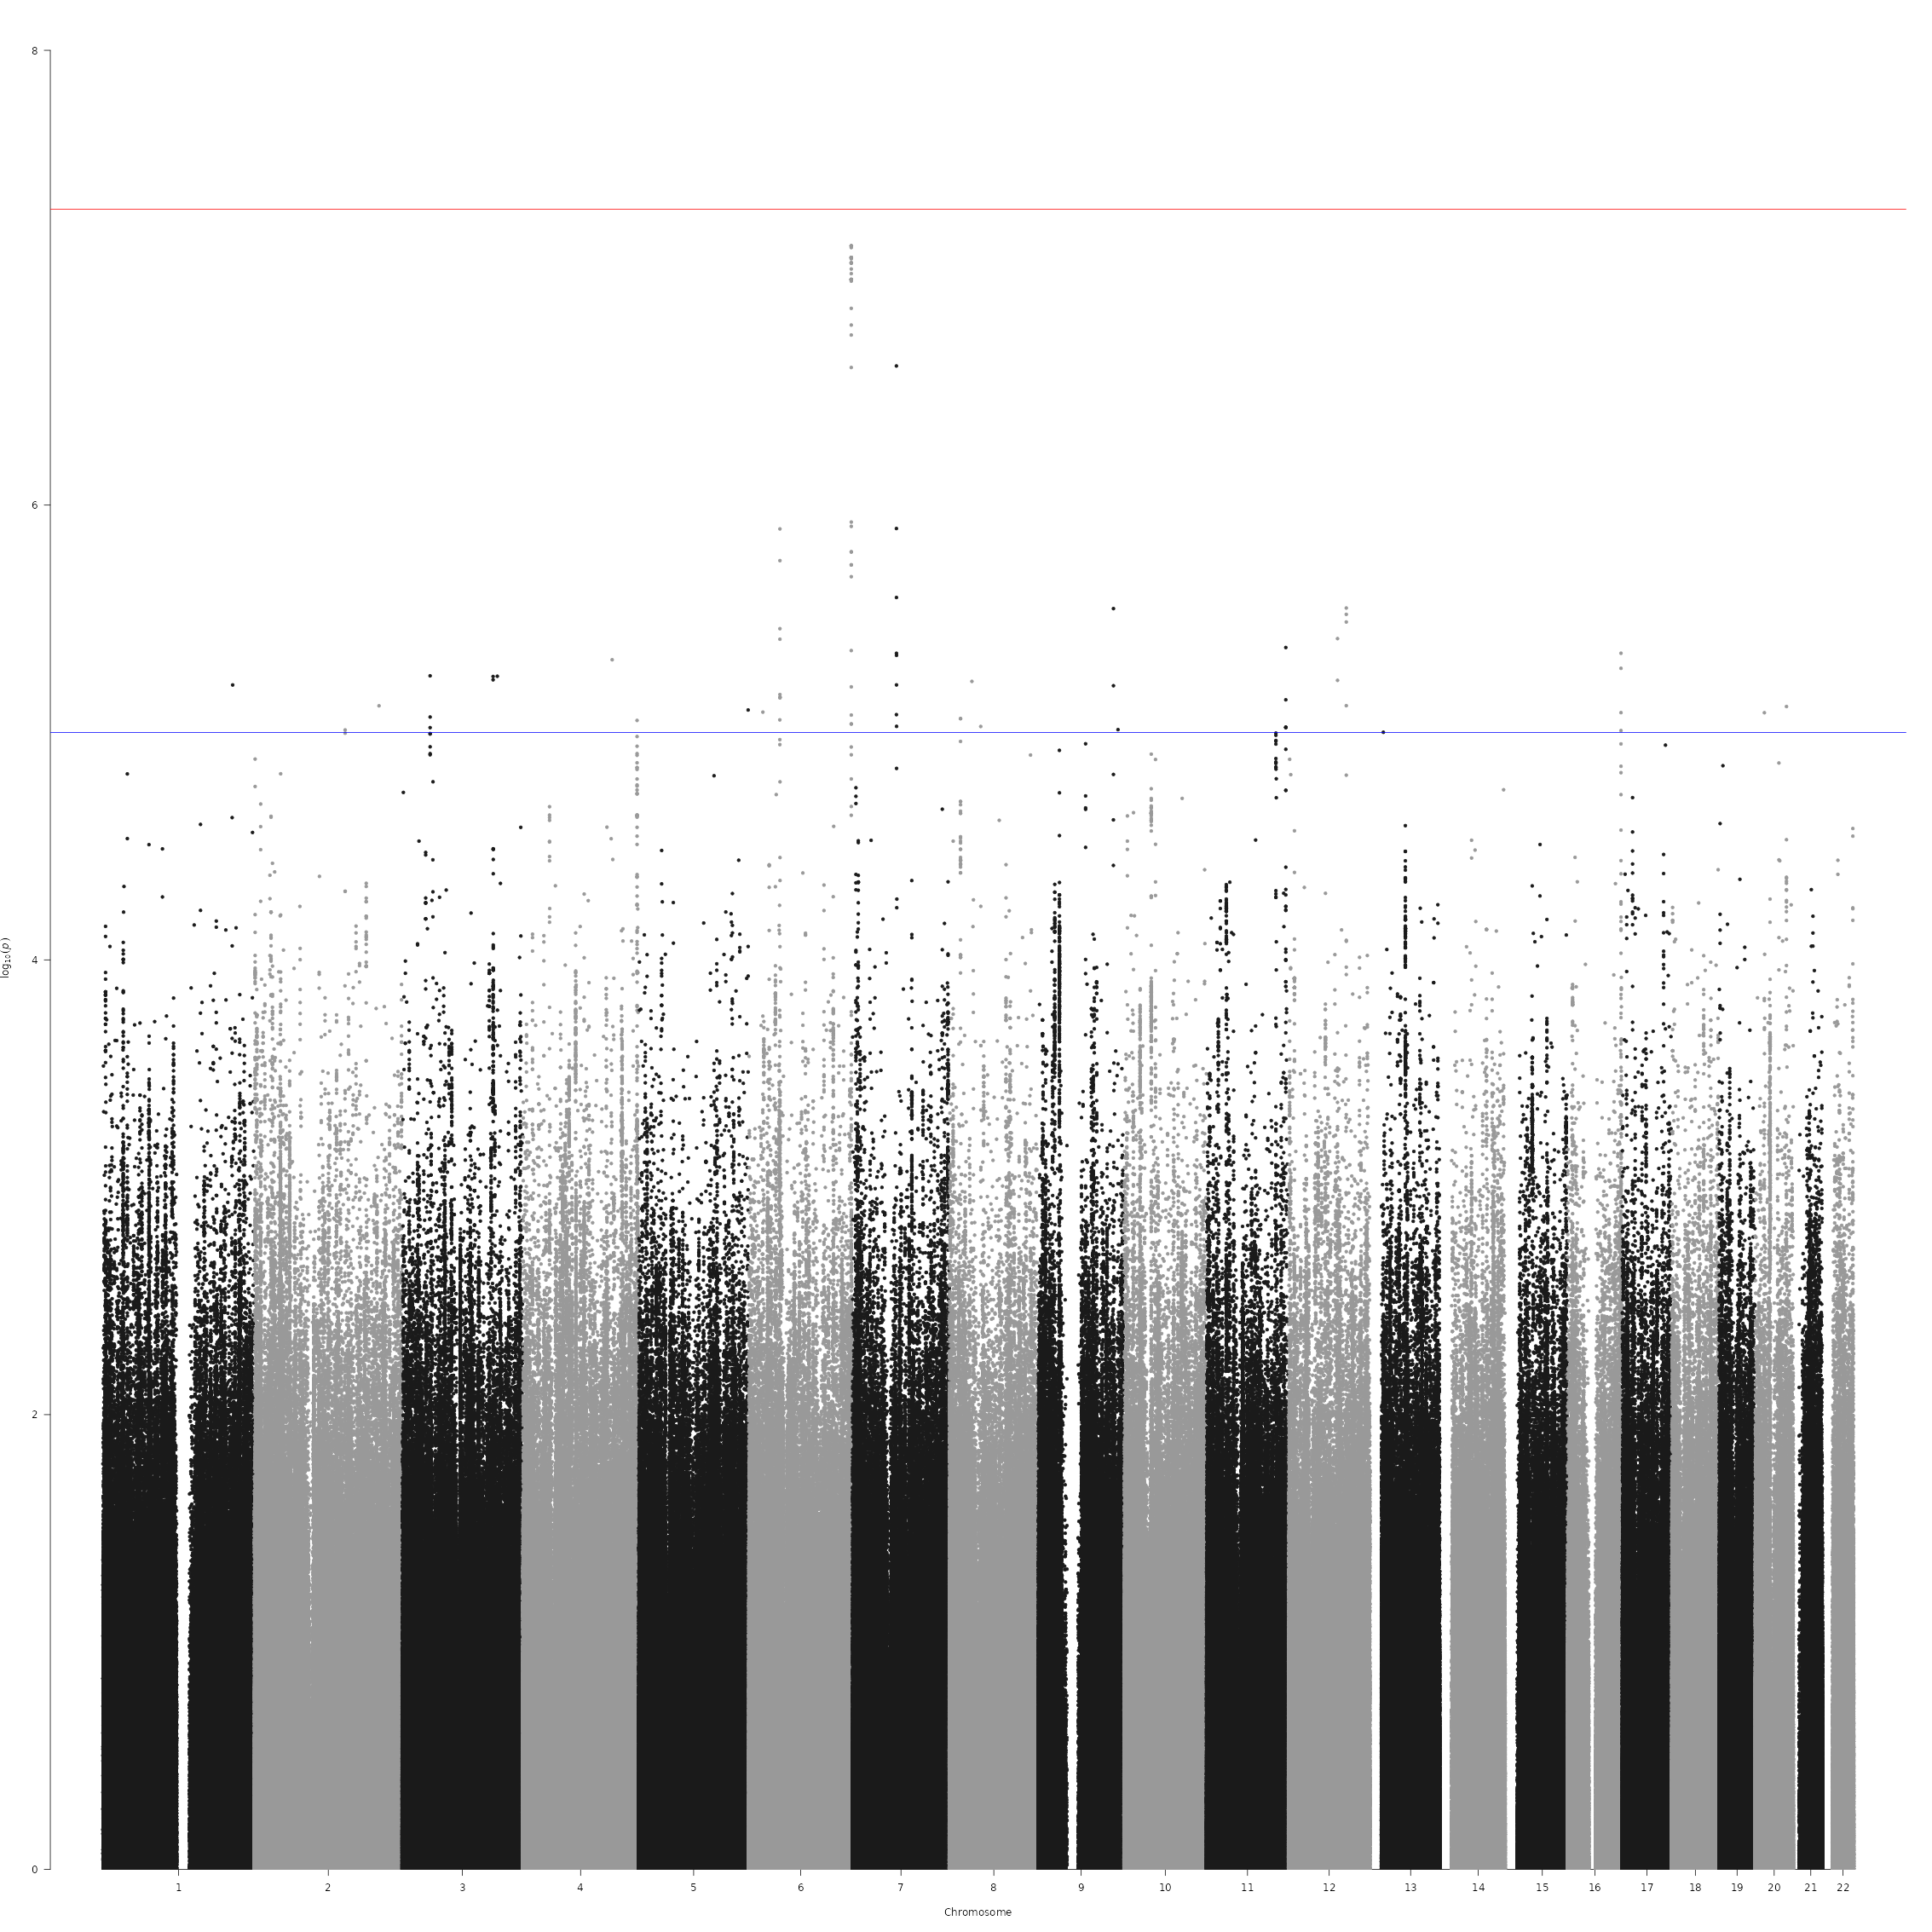
\includegraphics[width=\linewidth]{img/rssp_01.png}
    \caption{Manhattan plot for a simulated GWAS on 10,000 real genotypes for a trait with infinitesimal genetic architecture and $h^2=0.1$.  }\label{fig:gwas_01}
  \end{subfigure}
    \begin{subfigure}[t]{\textwidth}
    \centering
    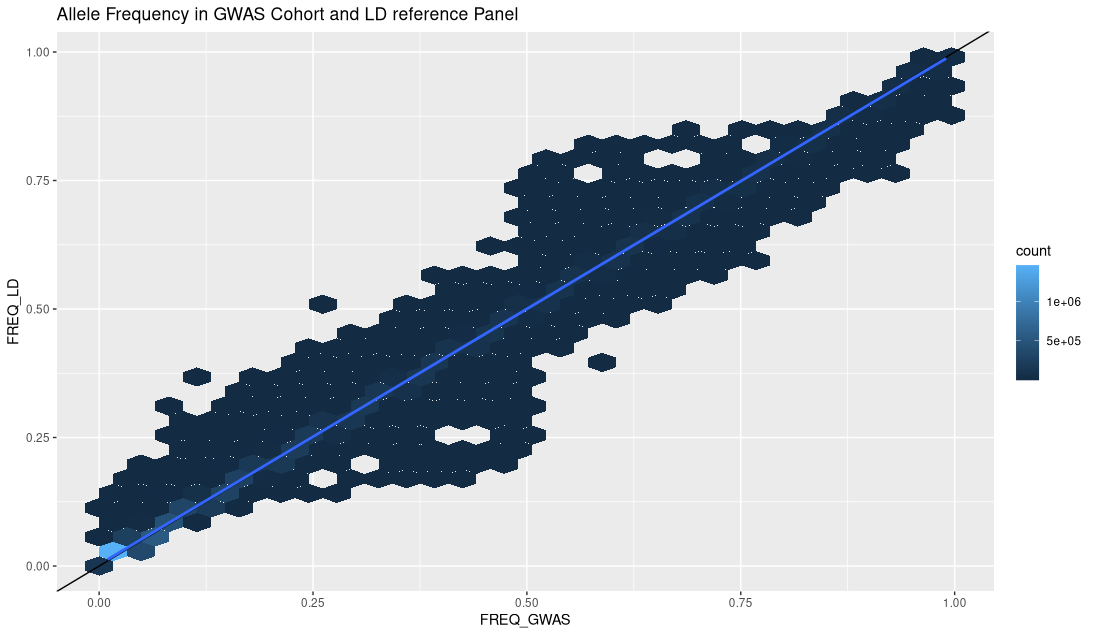
\includegraphics[width=\linewidth]{img/Allele_freq_match.png}
    \caption{Two dimensional histogram of non-reference allele frequency for variants in the GWAS cohort and LD reference panel.}\label{fig:gwas_01}
  \end{subfigure}
\end{figure}

\subsection{GWAS Simulations}
To estimate the effectiveness of RSSp at estimating heritability we simulated phenotypes and estimated GWAS summary statistics using a large employed a large-scale simulation of polygenic traits and GWAS summary statistics using real genotypes from the UK biobank.  We then employed state of the art individual-level data-based (\texttt{GCTA}\cite{GCTA}) and GWAS summary statistics-based (\texttt{ldsc}\cite{ldsc}) heritability estimation methods.  To make the simulations as realistic as possible, real individual-level genotypes were used.

Genotype data from individuals from the UK biobank were used as the basis of simulations. Two random non-overlapping subsets of 10,000 unlrelated individauls were randomly drawn (without replacement) from the 487,409 total individuals in the UK biobank dataset.  Both datasets were subset to include only the variants above 1 percent allele frequency in both subsets, resulting in 8,327,757 variants in total.

Causal variant effects and phenotypes traits were simulated using a modified version the \texttt{simu} software, a tool for simulating GWAS phenotypes based on real genotype data.  \texttt{simu} simulates causal effects from a normal distribution and uses the GCTA model of scaled genotypes.   For the infinitesimal simulation, 80 traits were simulated for 8 $h^2$ values from  0.1 to 0.8 in increments of 0.1, with 10 trait replicates
being simulated at each level of heritability.

After simulating the phenotype, heritability was estimated using GCTA's GCTA-GREML analysis, using a GRM constructed using the 8,327,757 variants and using 10 principal components as quantitative covariates. GWAS summary statistics for each simulated phenotype were then generated using GCTA's implementation of the \texttt{fastGWA} mixed linear model-based GWAS method, with the first 10 principle components used as quantiative covariates.

To estimate heritability using LD score regression, LD scores were generated on the 8,327,757 variants.  LD scores were generated from the genotypes used for the GWAS simulation (``in-sample''), and another set of LD scores were generated using the using the LD reference panel.  LD scores were estimated using \texttt{ldsc}, using a 1 centimorgan sliding window, as per the \texttt{ldsc} tutorial \cite{ldsctutorial} on the \texttt{ldsc} website.  The \texttt{pyrho} method applied to the British in England and Scotland (GBR) invdividuals from the 1000 genomes project\cite{1kg} was used in the estimation of the local recombination rate.  As we also wished to LD score regression was run four times on 

Finally, RSSp was 



The  one in-sample, set and  of using These GWAS summary statistics were then passed to \texttt{ldsc} or \texttt{RSSp}.


Estimates of $h^2$ from the individual-level data method GCTA were on average the closest to the true value of $h^2$ across every simulated value of $h^2$. 

% \subsection{RSSp outperforms LD score regression for in-sample and Simulation result}s\label{sec:orgdb752e7}


  \begin{figure}
      \centering
  \begin{subfigure}[t]{\textwidth}
    \centering
    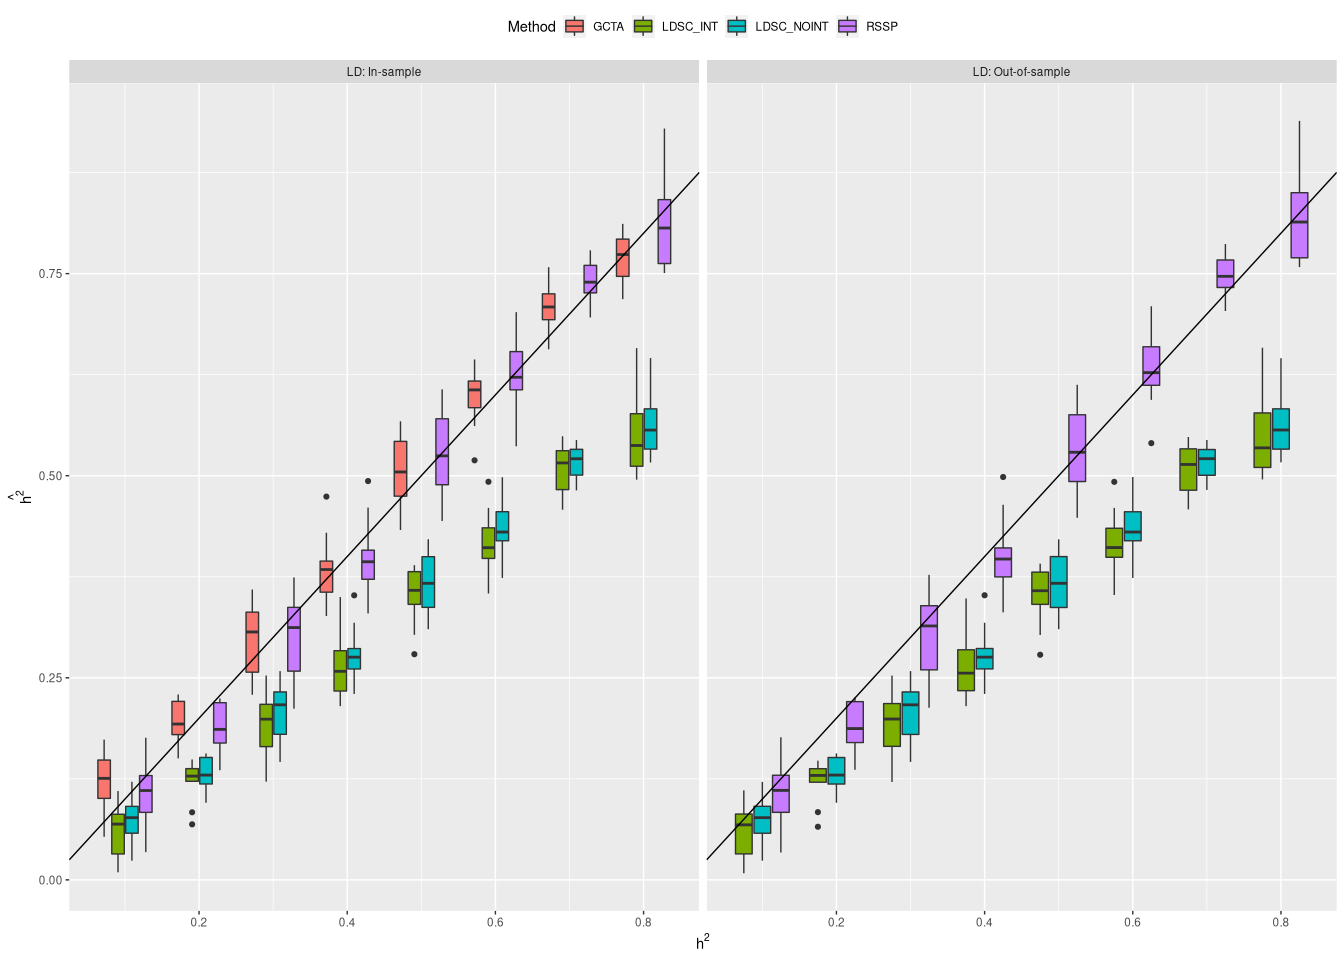
\includegraphics[width=.9\linewidth]{img/rsspnld_v_ldsc_v_gcta.png}
    \caption{$\hat{h^2}$ across 10 replicates across 8 values of $h^2$ for 4 methods of heritability estimation, estimated using either in-sample information, or an external reference LD panel. The black line along the diagonal represents a perfect 1 to 1 relationship between $\hat{h^2}$ and $h^2$.    The heritability estimation methods are as follows: 
    \texttt{GCTA} is the individual-level data single-component GREML, with 10 principal components used as continuous covariates (As GCTA requires individual level data, there can be no Out-of-sample result);
    \texttt{LDSC\_INT} is LD score regression \cite{ldsc} run with the default setting where the intercept term is allowed to vary; 
    \texttt{LDSC\_NOINT} is LD score regression run with a fixed intercept of 1;
    \texttt{RSSP} is RSSp (fit without a shrinkage estimator of LD)}\label{fig:rssp_method_comparison}
  \end{subfigure}
\end{figure}


\begin{table}
\begin{tabular}{l|l|r|r}
\hline
Method & LD & $\text{Bias}(h^2,\hat{h}^2)$ & $\text{MSE}(h^2,\hat{h}^2)$\\
\hline
GCTA & N/A & -0.0027508 & 0.0015073\\
\hline
RSSP\_NOSHRINK & In-sample & 0.0122161 & 0.0023406\\
\hline
RSSP\_NOSHRINK & Out-of-sample & 0.0161776 & 0.0025623\\
\hline
RSSP\_LDSHRINK & In-sample & 0.0240149 & 0.0030679\\
\hline
RSSP\_LDSHRINK & Out-of-sample & 0.0259495 & 0.0032210\\
\hline
LDSC\_NOINT & In-sample & -0.1280450 & 0.0213703\\
\hline
LDSC\_NOINT & Out-of-sample & -0.1280562 & 0.0213719\\
\hline
LDSC\_INT & In-sample & -0.1413375 & 0.0252106\\
\hline
LDSC\_INT & Out-of-sample & -0.1416675 & 0.0253203\\
\hline
\end{tabular}\label{tab:gwas_sim_ave_error}
\caption{Comparison of methods for heritability estimation on 8M variant simulation.  Bias was calculated over all simulated values of $h^2$ $\text{Bias}(h^2,\hat{h}^2)=\frac{1}{80}\sum_{i=1}^{10}\sum_{j=1}^{8}(\hat{h^2}_{i,j}-{h^2}_j)$.   Mean squared error (MSE) was calculated similarly: $\text{Bias}(h^2,\hat{h}^2)=\frac{1}{80}\sum_{i=1}^{10}\sum_{j=1}^{8}{(\hat{h^2}_{i,j}-{h^2}_j)}^2$.}
\end{table}

\subsubsection{Sparsity}

  \begin{figure}
      \centering
  \begin{subfigure}[t]{\textwidth}
    \centering
    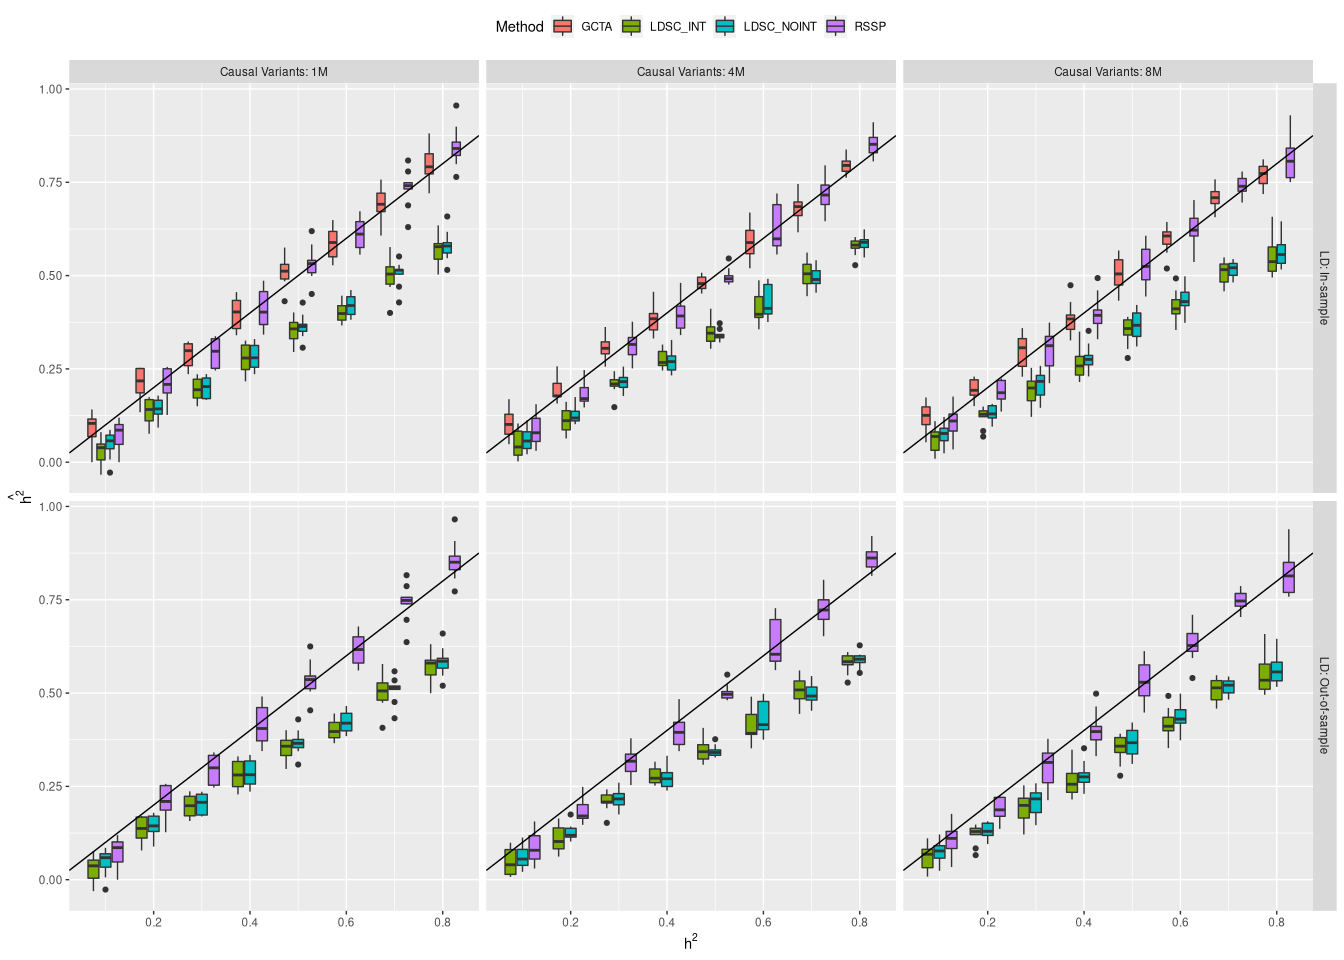
\includegraphics[width=.9\linewidth]{img/rssp_sparsity.png}
    \caption{$\hat{h^2}$ across 8 values of $h^2$ with 10 replicates each for for methods of heritability estimation. $\hat{h^2}$ was estimated using either in-sample information (top panels), or an external reference LD panel (bottom panels). Two sparse genetic architectures are represented along side the original infinitesimal model.  From left to right, causal variants contributing to $h^2$ numbered 1 million --- for a sparsity of 87.5\%, 4 million --- for a sparsity of 50\%, or 8 million, for a sparsity of 0\%.}\label{fig:rssp_sp_method_comparison}
  \end{subfigure}
\end{figure}


To asses the robustness of RSSp to model misspecification, we performed simulations which relaxed the infinitesimal assumption.  Using the 8,327,757 variant, 10,000 sample UK biobank dataset, we expanded our simulations to include sparse genetic architectures.  Starting with the original 8,327,757 variants, we created two randomly selected causal variant subsets, containing  4,163,878  and 1,040,970 variants.  Using these causal variant subsets, we simulated phenotypes under values of  $h^2$ from $0.1$ to $0.8$ in increments of $0.1$, from which we generated GWAS summary statistics on the original 8,327,757 variants.  For each value of $h^2$, and each of the two causal variant subsets we ran 10 simulations.  We then estimated heritability with each of the methods described previously.  The 

We found RSSp to be quite robust to sparsity at the three levels of sparsity simulated.  


\subsubsection{Hapmap 3}\label{sec:org0fa2c7f}

We hypothesized that the relatively poor performance of LD score regression was due to the very large number of causal variants relative to the sample size.  To test this hypothesis  We repeated the simulation using a 1,163,080 variant subset of our original 8,327,757 dataset.  These variants were drawn from the HapMap 3 reference panel\cite{hapmap3}.  It is recommended that users of LD score regression subset their GWAS summary statistics to the variants in the HapMap 3 reference panel\cite{ldsc}.  


\subsection{LD shrinkage estimators} 
To attempt to improve the estimate of LD, I used the LD shrinkage estimator developed by Wen and Stephens\cite{Wen_2010}, which uses an estimate of 
the recombination rate, as well an estiamte of the effective population size to improve the estimate of correlation between variants.
I implemented a standalone version of this shrinkage estimator in as R package called \texttt{LDshrink}. 

If \(\boldsymbol{X}\) is a \(n \times p\) matrix of genotype dosages, such that \(X_{i,j}\) represents the number of effect alleles at the \$j\$th variant in the \$i\$th individual, and \(\hat{\boldsymbol{\Sigma}}\) is the \(p \times p\)  the estimate of covariance between
variants, where:

\[\boldsymbol{\hat{\Sigma}} = (1-\theta)^2 \textbf{S}+\frac{\theta}{2} \left(1-\frac{\theta}{2}\right)\textbf{I}\],
where 
$$ S_{jk} = \begin{cases}
\text{Cov}(\boldsymbol{X}_{.j},\boldsymbol{X}_{.k}), \text{if } j=k \\
e^{-\frac{\rho_{jk}}{2n}}\text{Cov}(\boldsymbol{X}_{.j},\boldsymbol{X}_{.k}), \text{otherwise}\\
\end{cases} $$
and \(\rho_{jk}\) is an estimate of the population-scaled recombination rate between variants \(j\) and \(k\). After shrinkage, the covariance matrix is converted to a correlation matrix, and values below a given threshold (by default 0.001), are rounded down to 0 to induce sparsity in the resulting LD matrix.

Populating the \(\rho\) parameter requires an estimate of the population-scaled recombination rate at the the sites in the simulation.  The method \texttt{pyrho} is a fast, demography-aware method for inferance of fine-scale recombination rates, and is based on
the fused-LASSO\cite{Spence_2019}. The \texttt{pyrho} method applied to the British in England and Scotland (GBR) invdividuals from the 1000 genomes project\cite{1kg} were used in the estimation of the local recombination rate for the UK biobank simulations.



  \begin{figure}
      \centering
  \begin{subfigure}[t]{\textwidth}
    \centering
    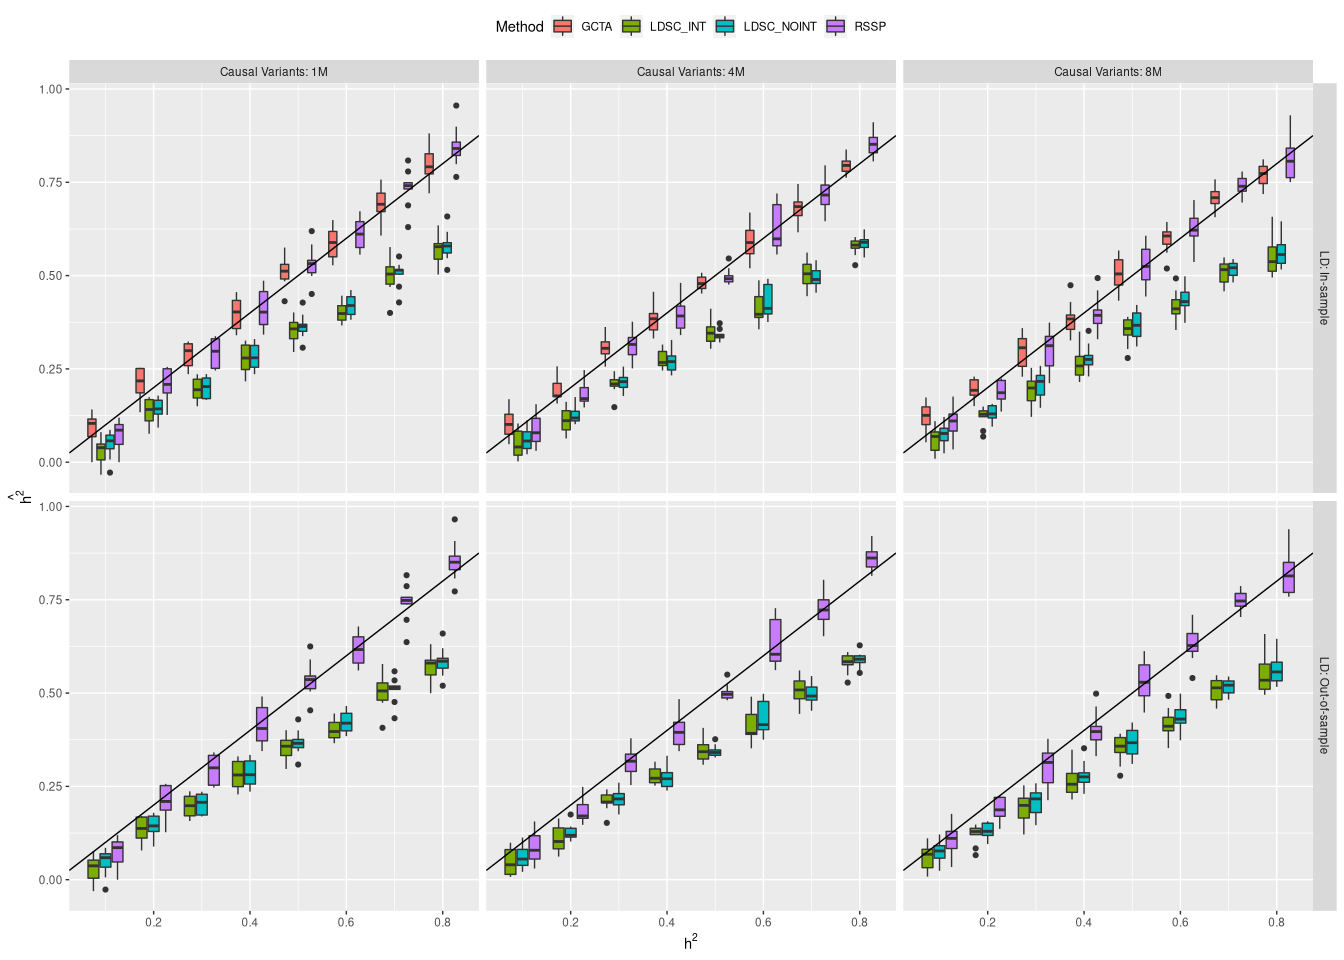
\includegraphics[width=.9\linewidth]{img/rssp_sparsity.png}
    \caption{Comparison of RSSp with and without an LD shrinkage estimator.  The original infinitesimal model was }\label{fig:rssp_sp_method_comparison}
  \end{subfigure}
\end{figure}





\section{Discussion}\label{sec:orge95691e}


In this study we show how SNP-heritability can be estimated using GWAS summary statistics and an out-of-sample reference LD panel with accuracy comparable to individual-level data methods, even when the number of variants exceeds the number of samples by several orders of magnitude.

Unlike previously described methods for estimation of LD from GWAS summary statistics, RSSp performs well under the block-diagonal approximation to the genome-wide LD matrix which allows for scalable estimate of SNP heritability on large numbers of variants. We further demonstrated the by partitioning the genome into approximately independent

While whe have shown that accurate estimation of SNP-heritability from GWAS summary statistics using an out-of-sample reference LD panel, there are some important caveats and future directions.  First, though there was no sample overlap between the GWAS cohort and the LD reference panel, both the cohort and the panel were randomly sampled from the same set of individuals.  The set of
variants used to simulate the GWAS were selected so that they were above 1 percent frequency in both the GWAS sample and in the LD reference panel.  If, for example, the 503 individuals in the \texttt{EUR} subset of the 1000 genomes dataset were used as a reference LD panel, the match between the datasets would have likely been poorer.

We investigated the effect of a shrinkage estimator on heritability estimates and found that it had little to no effect on estimates of heritability.  When the reference LD panel was the same size as the GWAS dataset

Previously studies had found that chunking the genome into chunks can introduce upward bias in heritability estimates, even when using in-sample LD estimates\cite{Hou_2019}.  While   The sub-chromosome block-wise approximation to the full LD matrix did not introduce significant upward bias in RSSp's heritability estimates in simulation, though.   In Hou et al, significant upward bias of heritability estimates were observed with block sizes as large as 4.3 megabases (when analyzing simulations based on a single 34 megabase chromosome).  The median block size of the ldetect LD blocks is much smaller, at approximately 1.5 megabases, and yet RSSp did not show appreciable inflation.

We have demonstrated that LD score regression is biased under truly infinitesimal genetic architectures.  Even with the intercept fixed at zero, we found in our simulations
that LD score regression consistently underestimates $h^2$, and the amount LD score regression underestimates $h^2$ increases as $h^2$ increases.
and this is understimate is
heritability is not biased.
We find that in the absence of population structure, LD score regression 
Our simulations did not explore the In the absence of 






